\documentclass[a4paper,12pt]{report}

% ================== PAQUETES ==================
\usepackage[a4paper, top=2.5cm, bottom=2.5cm, left=3cm, right=3cm]{geometry}
\usepackage{float}
\usepackage{pgfplots}
\usepackage{graphicx}
\usepackage{lettrine}
\usepackage{ragged2e}
\usepackage{microtype}
\usepackage{amsmath, amssymb}
\usepackage{booktabs}
\usepackage{longtable}
\usepackage{siunitx}

\usepackage[dvipsnames]{xcolor}
\usepackage{pagecolor}

\usepackage{tikz}
\usepackage{pgfplots}
% compat eliminado para evitar conflictos en MiKTeX

\usetikzlibrary{arrows.meta}

\usepackage{fancyhdr}

% hyperref SIEMPRE al final
\usepackage{hyperref}

% ================== CONFIGURACIÓN ==================
\sisetup{
  round-mode=places,
  round-precision=6
}

\setlength{\parindent}{0pt}
\setlength{\parskip}{6pt}
\setlength{\headheight}{16pt}

% ================== ENCABEZADOS ==================
\pagestyle{fancy}
\fancyhf{}
\fancyhead[L]{\leftmark}
\fancyfoot[C]{\thepage}
\renewcommand{\headrulewidth}{0.4pt}
\renewcommand{\footrulewidth}{0.4pt}

% ================== HIPERVÍNCULOS ==================
\hypersetup{
    colorlinks=true,
    linkcolor=MidnightBlue,
    urlcolor=RoyalBlue,
    citecolor=BrickRed
}

% ================== DOCUMENTO ==================
\begin{document}

% ================== PORTADA ==================
\newgeometry{top=4cm, bottom=4cm, left=4cm, right=4cm}
\begin{titlepage}
\pagecolor{MidnightBlue}
\color{white}
\centering

\vspace*{2cm}

{\Huge\bfseries Apuntes de Cálculo Multivariable}\\[2.5cm]

{\Large Moisés Hernández Pacheco}\\[6cm]

{\color{SkyBlue}\Large Matemáticas Aplicadas \& Computación}\\[1cm]
{\large Universidad Nacional Autónoma de México}\\[0.5cm]
{\large FES Acatlán}

\vfill

\begin{tikzpicture}[xscale=3]
\draw[white, thick] (-2,0) -- (2,0);
\draw[white, thick] (-2,-0.5) -- (2,-0.5);
\end{tikzpicture}

\vfill
{\large \today}

\end{titlepage}
\restoregeometry
\pagecolor{white}
\color{black}

% ================== ÍNDICE ==================
\hypersetup{linkcolor=black}
\tableofcontents
\newpage

% ================== PIES CON ENLACE ==================
\fancyfoot[R]{\hyperlink{toc}{Ir al índice}}

% ================== CONTENIDO ==================
\part{Introducción al Cálculo Multivariable}

\chapter{Funciones Multivariables}

\section{Introducción intuitiva}

Recordando las funciones vistas en cursos previos de cálculo, normalmente trabajábamos con funciones de una sola variable, por ejemplo:
\[
f(x) = x^2
\]

Aquí, $x$ representa la variable independiente. A este tipo de expresiones las llamamos \textbf{funciones de una variable}.

Intuitivamente, una \textbf{función multivariable} es aquella que depende de más de una variable. Un ejemplo sencillo es:
\[
f(x,y) = 3x^2 + y
\]

También existen funciones cuyo resultado no es un número real, sino un vector. Por ejemplo:
\[
f(x,y) =
\begin{bmatrix}
3x \\[4pt]
5y^2
\end{bmatrix}
\]

En este caso, la entrada $(x,y)$ puede interpretarse como un \textbf{punto en el plano cartesiano}.

\begin{figure}[H]
\centering
\resizebox{0.4\textwidth}{!}{
\begin{tikzpicture}
\begin{axis}[
    axis lines = middle,
    xmin=0, xmax=10,
    ymin=0, ymax=6,
    xlabel={$x$},
    ylabel={$y$},
    tick style={draw=none},
    xticklabels=\empty,
    yticklabels=\empty
]
\addplot+[
    only marks,
    mark=*,
    mark size=3
] coordinates {(5,3)};
\end{axis}
\end{tikzpicture}
}
\caption{Punto $(x,y)$ en el plano}
\end{figure}

Sin embargo, a diferencia de las funciones de una sola variable, las funciones multivariables suelen representarse en tres dimensiones o más. 


Aquellas funciones que dependen de dos variables de entrada pueden graficarse en tres dimensiones; no obstante, cuando una función tiene más de dos variables independientes, \textbf{no es posible representarla gráficamente de la forma tradicional}. En estos casos, se emplean distintos métodos y herramientas que permiten obtener una idea de su comportamiento y estructura, los cuales se estudiarán más adelante.
\\

\begin{figure}[H]
\centering
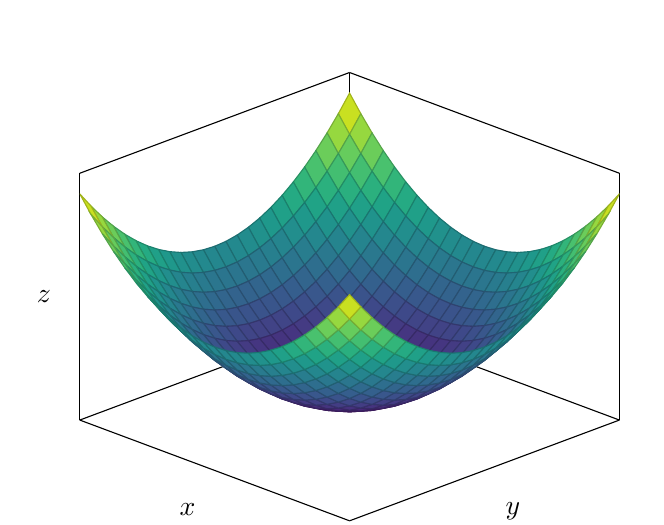
\begin{tikzpicture}
\begin{axis}[
    view={45}{30},
    xlabel={$x$},
    ylabel={$y$},
    zlabel={$z$},
    zlabel style={rotate=270},
    tick style={draw=none},
    xticklabels=\empty,
    yticklabels=\empty,
    zticklabels=\empty,
    domain=-2:2,
    y domain=-2:2,
    samples=25,
    colormap/viridis,
]
\addplot3[
    surf,
]
{x^2 + y^2};
\end{axis}
\end{tikzpicture}
\caption{Superficie $z = x^2 + y^2$}
\end{figure}



Como se verá más adelante, las funciones de dos o más variables, cuyas gráficas corresponden a superficies en tres o más dimensiones, pueden visualizarse en dos dimensiones mediante procesos de proyección o “aplanamiento”. Este enfoque permite analizar su comportamiento de manera más accesible, sin perder información relevante, y conduce igualmente a resultados de gran interés.


\begin{figure}[H]
\centering
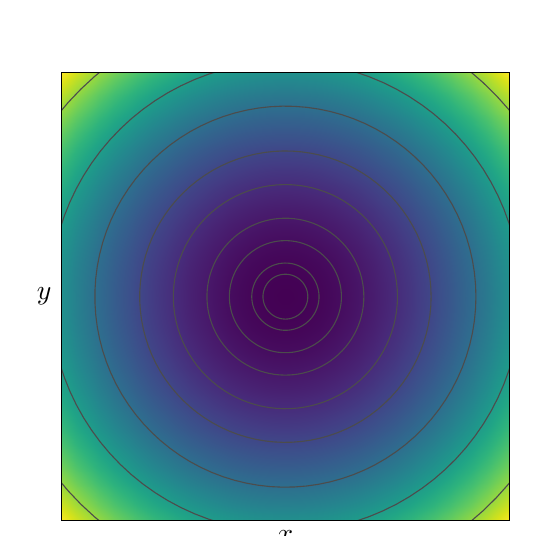
\begin{tikzpicture}
\begin{axis}[
    view={0}{90},
    axis equal image,
    enlargelimits=false,
    xlabel={$x$},
    ylabel={$y$},
    ylabel style={rotate=270},
    xtick=\empty,
    ytick=\empty,
    ztick=\empty,
    xmin=-2, xmax=2,
    ymin=-2, ymax=2,
    domain=-2:2,
    y domain=-2:2,
    samples=60,
    colormap/viridis,
]

% Superficie con degradado suave que cubre todo el fondo
\addplot3[
    surf,
    shader=interp,
]
{x^2 + y^2};

% Curvas de nivel más densas
\foreach \r in {0.2, 0.3, 0.5, 0.7, 1.0, 1.3, 1.7, 2.1, 2.6} {
    \addplot3[gray!60!black, thin, domain=0:360, samples=100, samples y=0]
        ({\r*cos(x)}, {\r*sin(x)}, 0);
}

\end{axis}
\end{tikzpicture}
\caption{Curvas de nivel de la función $z = x^2 + y^2$}
\end{figure}









\end{document}
